%%----------------------------------------------------------------------
%%----------------------------------------------------------------------
\makeatletter\@openrightfalse
\chapter{Story So Far}
\@openrighttrue\makeatother

We pick up our tale in the future...

\bigskip
\begin{center}  
\begin{tabular}{L{6in}}
  \arrayrulecolor{LineColor}\hline\\
  {\it
  The Virtue is the greatest civilization ever arisen in the galaxy.
  More than a species, more than an empire, more than a philosophy; The
  Virtue is a way of being.  Its culture and technology
  are unsurpassed.  Its will is absolute.  The Virtue is perfect.

  \bigskip
  The Virtue \emph{was} perfect.

  \bigskip
  It has been three hundred years since The Virtue fought Humanity.  Their
  pacification forces were smashed, but at great cost to the human
  defenders.  Earth is a barren husk.  Its mighty war fleets have
  vanished, scattered to the solar winds if not lost entirely.  A paltry
  few survivors' colonies have integrated into the ignored, disordered,
  minor societies along the fringe worlds and outlaw regions at the edge
  of The Virtue's control, enduring as best they can in the shadow of the
  colossus.

  \smallskip
  The Virtue, for its part, has retreated into itself.  Effects of that
  failed conquest echo still, slowly rippling across the staid society.
  For the first time in millennia, murmurs of disquiet have been heard
  in the governance enclaves.  Questions flitter across the dataplane.
  How could a perfect society be defeated by such an unenlightened race?
  In a universe where everything is known, what could be unknown?

  \smallskip
  Spawned from this moral crisis, disparate elements on the perimeter of
  The Virtue's space have begun fomenting open rebellion.  Branding themselves
  the Coalition of the Free, their messages have appeared across
  message boards and even hastily graffitied in public spaces on the
  outer worlds, praising a new virtue:

  \bigskip
  \centerline{The virtue of freedom.}
  }
  \\
  \arrayrulecolor{LineColor}\hline\\
\end{tabular}
\end{center}

\section{The Past}

The~2016~40k Narrative continues the ongoing NOVA story of The Virtue
and Humanity.

\paragraph{NOVA 2012: First Contact.}  After a brush with global
nuclear war in~2194, humanity stepped back from the brink.  The
millennia-old dreams of scholars, tyrants, and preachers became a
reality as all the people of Earth finally set aside their
differences.  That peace was shattered a mere eighteen years later
when thousands of alien craft struck the planet without warning.
Millions died before any response could even begin.  Eventually though
a resistance formed.  Taking its last stand in Washington, D.C., the
defenders were dumbfounded when the invaders inexplicably retreated.

%\clearpage
\noindent\begin{minipage}[c]{(0.6\linewidth)-1em}%\vbox to 0pt{}
\paragraph{NOVA 2013: Cataclysm.}  Learning what they could from alien
captives and technology left behind, humanity strove to rebuild and
prepare.  Their caution was well founded: In~2312, one hundred years
to the day of the first invasion, the invaders struck again.  Against
much improved resistance and plagued by doubts, they once more though
faltered even as millions died.  Faced with defeat, their commander
rammed his flagship into Earth in a final ignominious gesture,
igniting its antimatter cores in the planetary mantle.  The blast and
shockwaves killed billions, with billions more lost in catastrophic
aftereffects.  Humanity survived merely through those few population
centers shielded enough to outlast the trauma.

\bigskip
\paragraph{NOVA 2014: Descension.} Regrouping in the aftermath,
humanity began a two-pronged offensive.  Space fleets began pushing
outward from Earth, learning much about the invaders and from where
they had come.  Forces on Earth meanwhile attempted to cleanse the
planet of the alien warriors still fighting on it and begin to restore
the environment.  This effort however was a grim one.  The planet had
taken so much damage, and numerous invaders were still extant on the
surface.  Eventually the cold truth became clear and inevitable: Earth
was no longer a safe home for humanity.
\end{minipage}\hfill%
\begin{minipage}[c]{0.4\linewidth}%\vbox to 0pt{}
  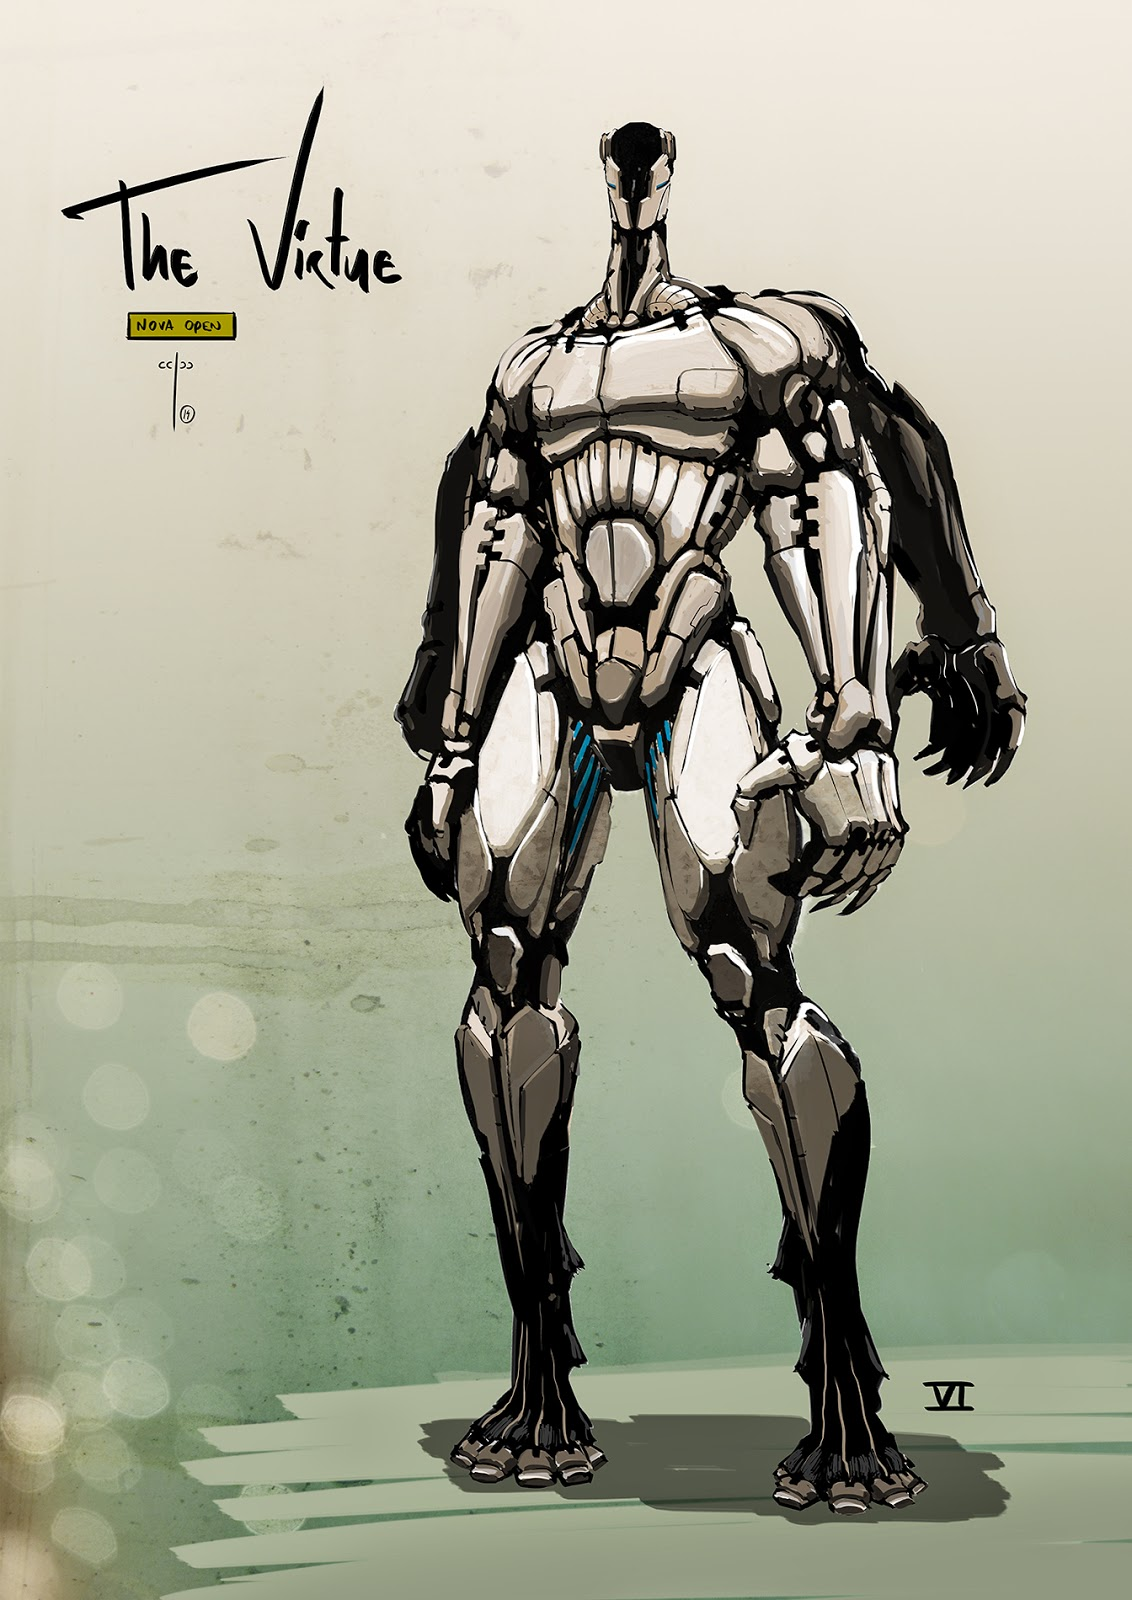
\includegraphics[width=\linewidth]{art/characters/virtue-warrior.jpg}
\end{minipage}

\paragraph{NOVA 2015: Ascension.}  Building on their successes in
space, humanity's remaining military focused on the war in the void.
A massive invader space station was discovered and captured, yielding
access to the Bend gates through which they warped time and space to
travel across the stars.  Meanwhile, ground forces fought to rescue
and protect what remnants of Earth's remaining population they could.
Although a tremendous evacuation was enacted, its scale was tragically
dwarfed by all those necessarily left behind.  After huried but
intense debate, humanity was split.  Some armed forces returned to
Earth to salvage the planet if at all possible. The majority though,
labeling itself the Phoenix fleet, took in the evacuees, closed and
destroyed the Bend gate inbound to Earth, and launched on an exodus to
colonize other worlds...

\section{The Virtue}

The alien invaders that beset Earth in~2212 were eventually revealed
as warriors of The Virtue.  For thousands of years The Virtue have
ruled much of the galaxy, encompassing innumerable worlds and species.
Built on fundamental, inarguable virtues and morals, over millenia the
tenets of their society have progressed to become part of their
collective genetic makeup itself.  The Virtue society can do no wrong,
and its citizens need not question if they might do wrong in following
its dictates.

As such, none of The Virtue warriors encountered in the fighting over
Earth had ever questioned their task.  For all of known history The
Virtue had stood in judgement over all the fledgeling races of the
galaxy.  As those species reached the threshold of relevance, The
Virtue applied a standard protection and inclusion protocol: Were they
a destructive cancer to be eliminated, or a desirable new element to
be incorporated into The Virtue?  Humanity was simply found wanting,
no further explanation needed.

But those colossal, four-armed warriors encountered on Earth are but
one face of The Virtue, just one of its militaries tasked with
pacifying young races.  The Virtue society is truly vast, and deep
within its governance structures another conclusion had been derived
from the protocols.  From that initial crack, the events at Earth have
slowly emerged as a growing fault line in the very foundations of The
Virtue society.  Never before had The Virtue been turned back from its
objectives, least of all by such an insignificant young race as
Humanity.  For those that have truly considered the implications, the
sheer outrageousness of the defeat calls into question the very
essence of The Virtue.  Eons-old civilizations don't fall often or
easily, but when they do, it comes from doubts such as these.

\section{The Free}

Three centuries later, those doubts have flickered into wisps of open
dissent.  On a far flung edge of The Virtue's territory, a group
labeling itself the Coalition of the Free has developed as if from
nowhere and taken increasingly provocative actions.  It began on the
public forums of the dataplane, messages citing discouraged texts and
raising questions from hijacked sockets beamed into from unrecognized
space.  Emboldened by faint stirrings of doubt, Coalition-sponsored
covert meetings began appearing on worlds of The Virtue themselves,
disseminating their message and recruiting to their beliefs.
Recently, the most brazen cells have shockingly defaced government
buildings and even sabotaged pacification assets.

Operating within the strictures of their philosophy and being, local
Virtue officiants have been unable to truly process and address these
events.  Most hazily interpret the Coalition of the Free as outside
attackers feared to be on the verge of invading The Virtue space.
Although almost wholly unprecedented, this is at least a largely
understandable concept.  Deeper, darker corners of The Virtue though
better understand the true threat.  Worse, they suspect and fear that
the Coalition has been helped by traitorous elements within the
government.  Elements that might even explain mysterious aspects of
the defeat at Earth.

Within the Coalition of the Free itself, hopes and passions run
rampant as wildfire.  Twinned rumors circulate among its cells.  One
tells of the discovery of a mighty weapon with which to fight The
Virtue.  Another posits an opportunity in the near future to make a
daring strike at a very pillar of The Virtue's control in the
region.  True or false, the whole of its decentralized structure
buzzes with activity and preparation...

\section{The Future}

The NOVA 2016 40k Narrative begins at this moment on the precipice,
and players must choose a side:

\begin{center}
\begin{minipage}[c]{1in}
  \fbox{
\includegraphics[width=\linewidth]{art/icons/free.pdf}}
\end{minipage}%
\hspace{2em}%
\begin{minipage}[c]{4in}
  Fight for \textbf{Humanity} as a secret leader and instigator of the
  Coalition of the Free, striving to capture the rumored weapon and
  strike at The Virtue to preserve your race and release many others
  from its oppressive grip.
\end{minipage}

\bigskip
  
\begin{minipage}[c]{4in}
  Command a military of \textbf{The Virtue}, directing a pacification
  force dispatched to uncover the traitor, quell rebellion, hunt down
  outside agitators, and restore peace and order by smashing the
  Coalition of the Free decisively.
\end{minipage}%
\hspace{2em}%
\begin{minipage}[c]{1in}
  \fbox{
\includegraphics[width=\linewidth]{art/icons/virtue.pdf}}
\end{minipage}
\end{center}
